\chapter{Medicion de distorción armónica}
\section{Medición}
Utilizando el analizador de espectros, se midió la distorsión armónica del generador de funciones Agilent(modelo)
con una señal senoidal de $0.7\si{\mega\hertz}$ y $250\si{\milli\volt} pp$.

Para calcular la distorsión armónica total (THD) medida con el analizador, se utilizaron las ecuaciones \ref{eq:THD}
y \ref{eq:P_k}.
\begin{equation}
    THD=\frac{\sum_{j=1}^{n} P_j}{\sum_{i=0}^{n} P_i}
    \label{eq:THD}
\end{equation}

\begin{equation}
    P_k[\si{\milli\watt}]= 1\si{\milli\watt} * 10^{P_k[dBm]/10}
    \label{eq:P_k}
\end{equation}

Entonces,

\begin{equation*}
    P_0 = 123 mW;P_1 = 123 mW;P_2 = 123 mW
\end{equation*}

\begin{equation}
    \Rightarrow THD = Ans
\end{equation}

Con las mediciones obtenidas del analizador (figuras \ref{fig:espectro_agilent} y \ref{fig:espectro_instek}) y cácluclos anteriores y utilizando otros generadores de funciones, se obtuvo la siguiente tabla:

\begin{table}[h]
    \begin{center}
        \begin{tabular}{|c|c|c|c|c|c|c|c|}
            \hline
            Modelo & $P_0 (mW)$ & $P_1 (mW)$ & $P_2(mW)$ & $P_3(mW)$ & $P_4(mW)$ & $THD(\%)$ & $THD_{Fab}(\%)$ \\
            \hline
            Agilent  & 0.0316 & 1.995e-6 & 1e-9 & - & - & 0.006 & 0.04 \\
            Picotest & 0.0437 & 2.399e-6 & 1e-9 & - & - & 0.005 & 0.06 \\
            Instek   & 0.1820 & 6.310e-5 & 2.089e-5 & - & 1.514e-6 & 0.047 & 1 \\
            \hline
        \end{tabular}
        \caption{Mediciones de Potencias en el analizador}
        \label{tab:ejmeas}
    \end{center}
\end{table}

\begin{figure}[ht]
    \begin{center}
        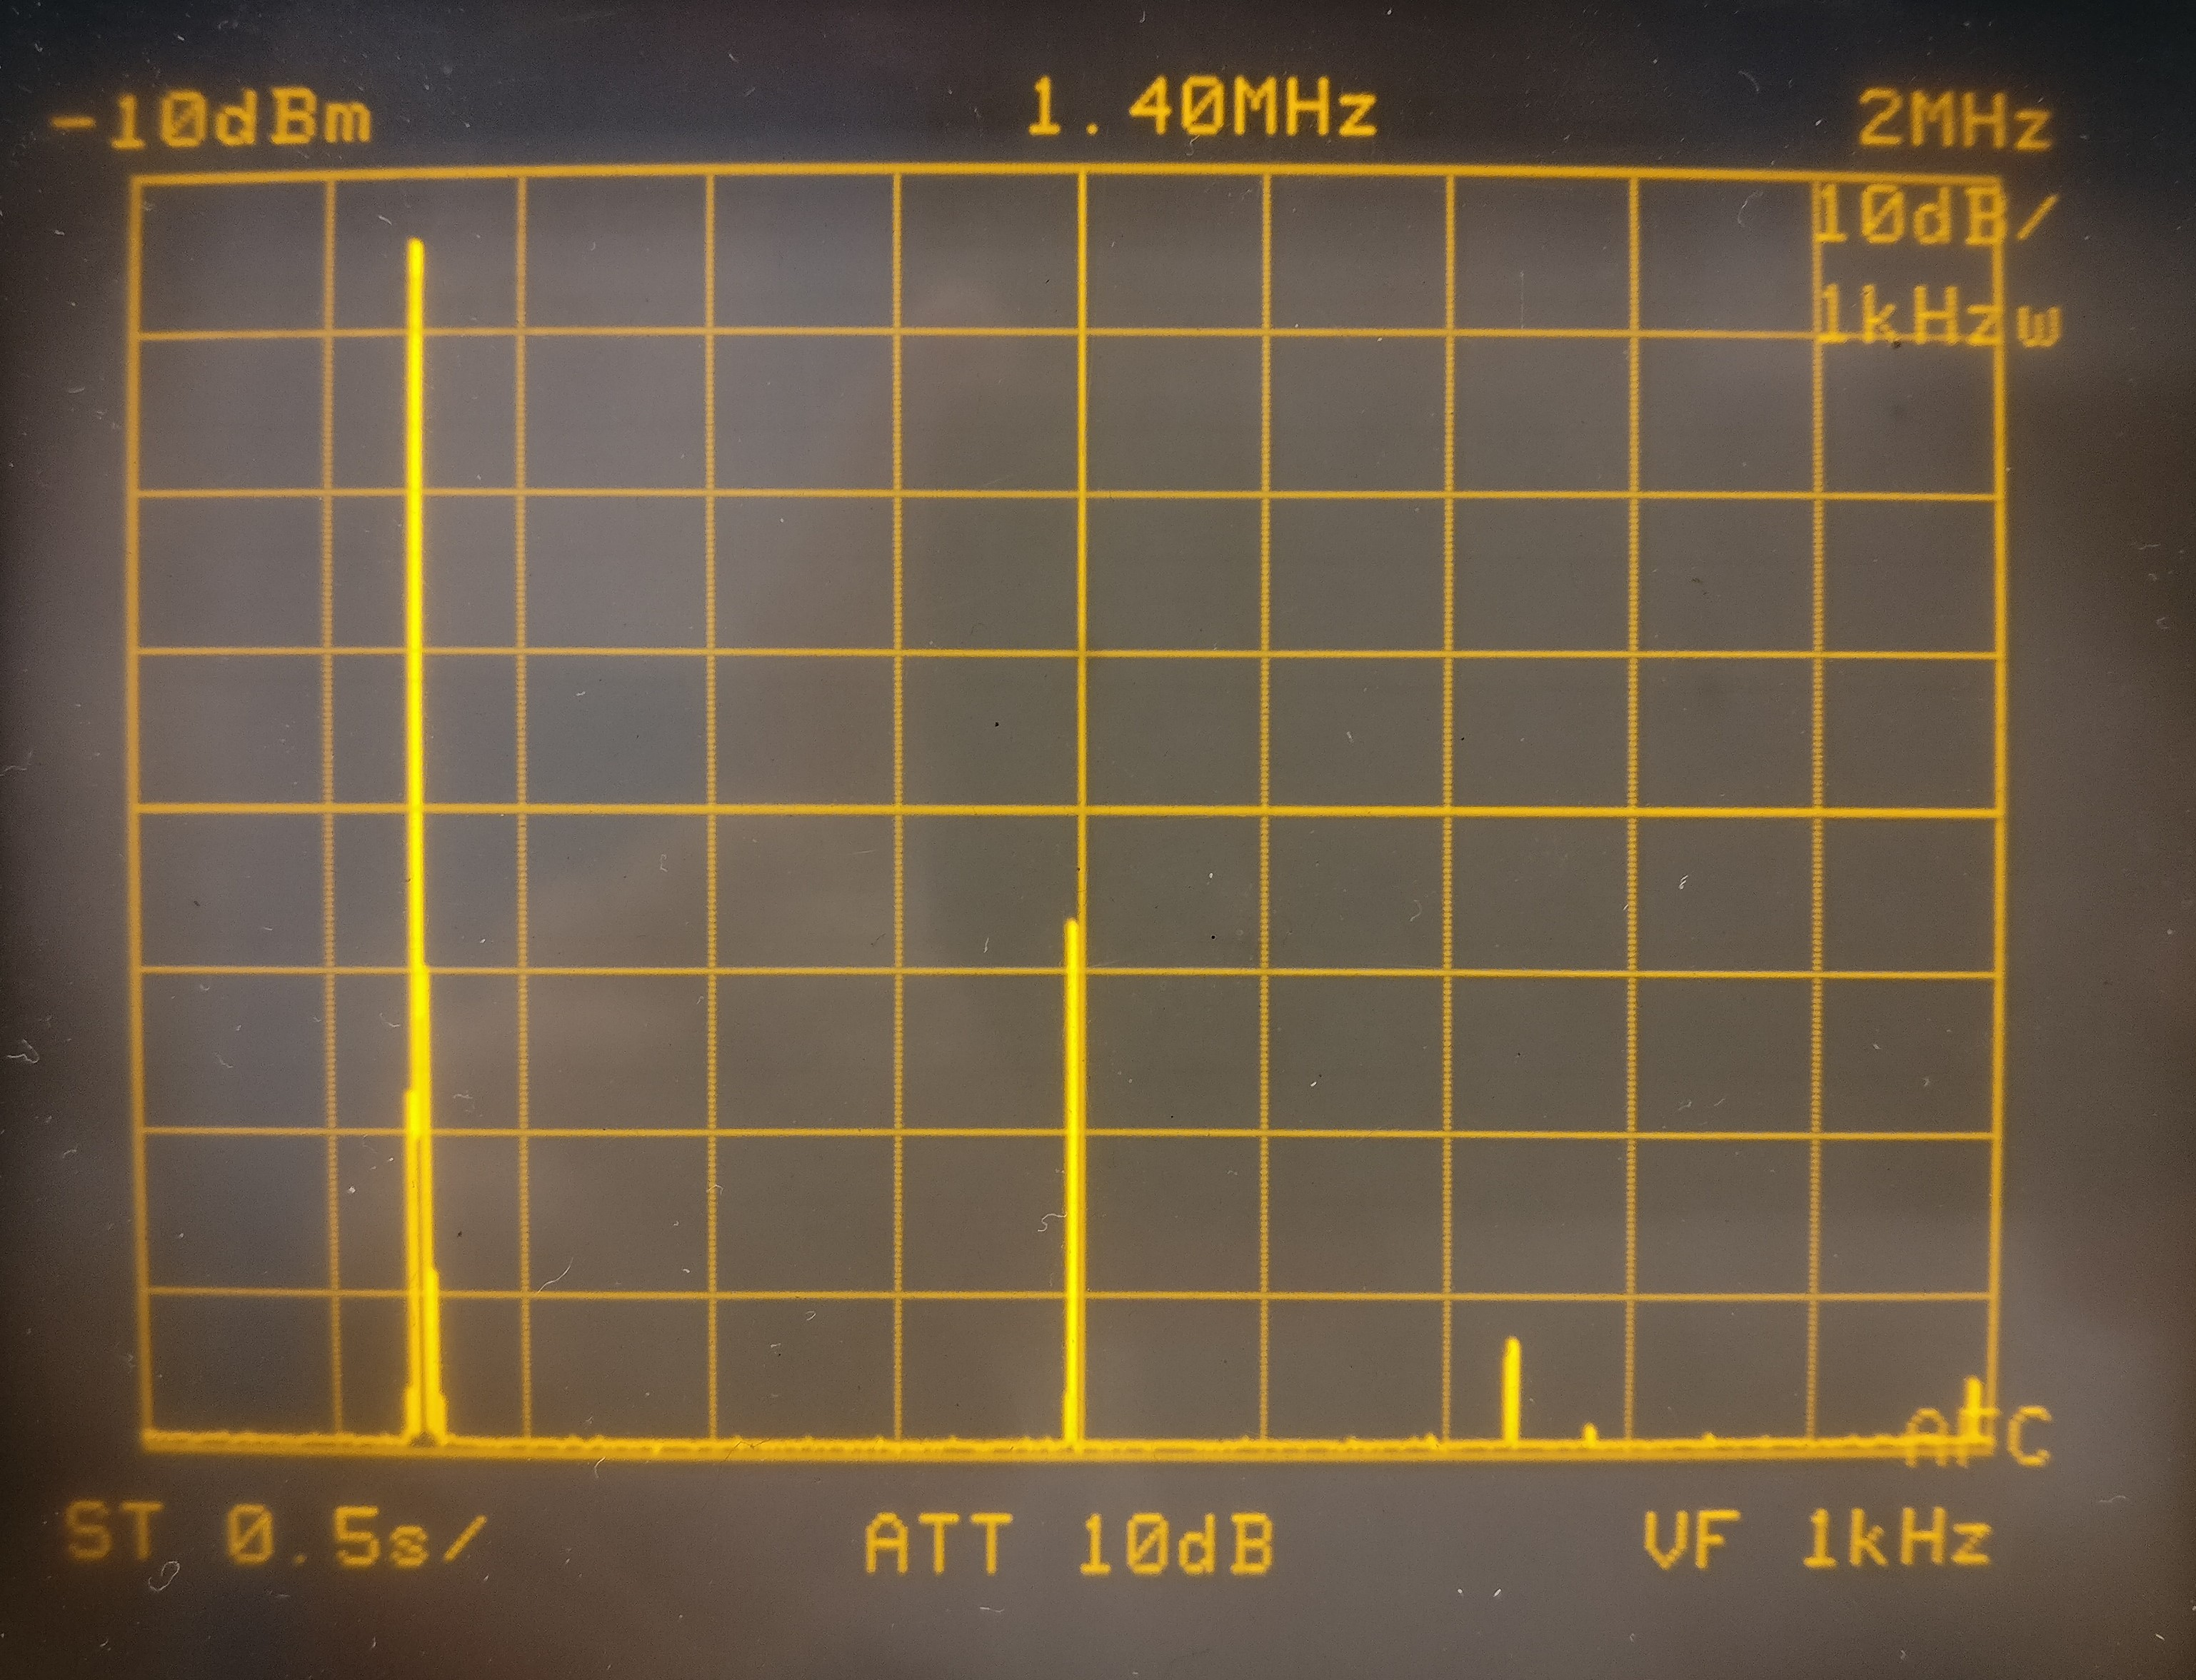
\includegraphics[width=0.5\linewidth]{contenido/img/espectro_senoidal.jpg}
        \caption{Espectro de la senoidal en el generador Agilent}
        \label{fig:espectro_agilent}
    \end{center}
\end{figure}

\begin{figure}[ht]
    \begin{center}
        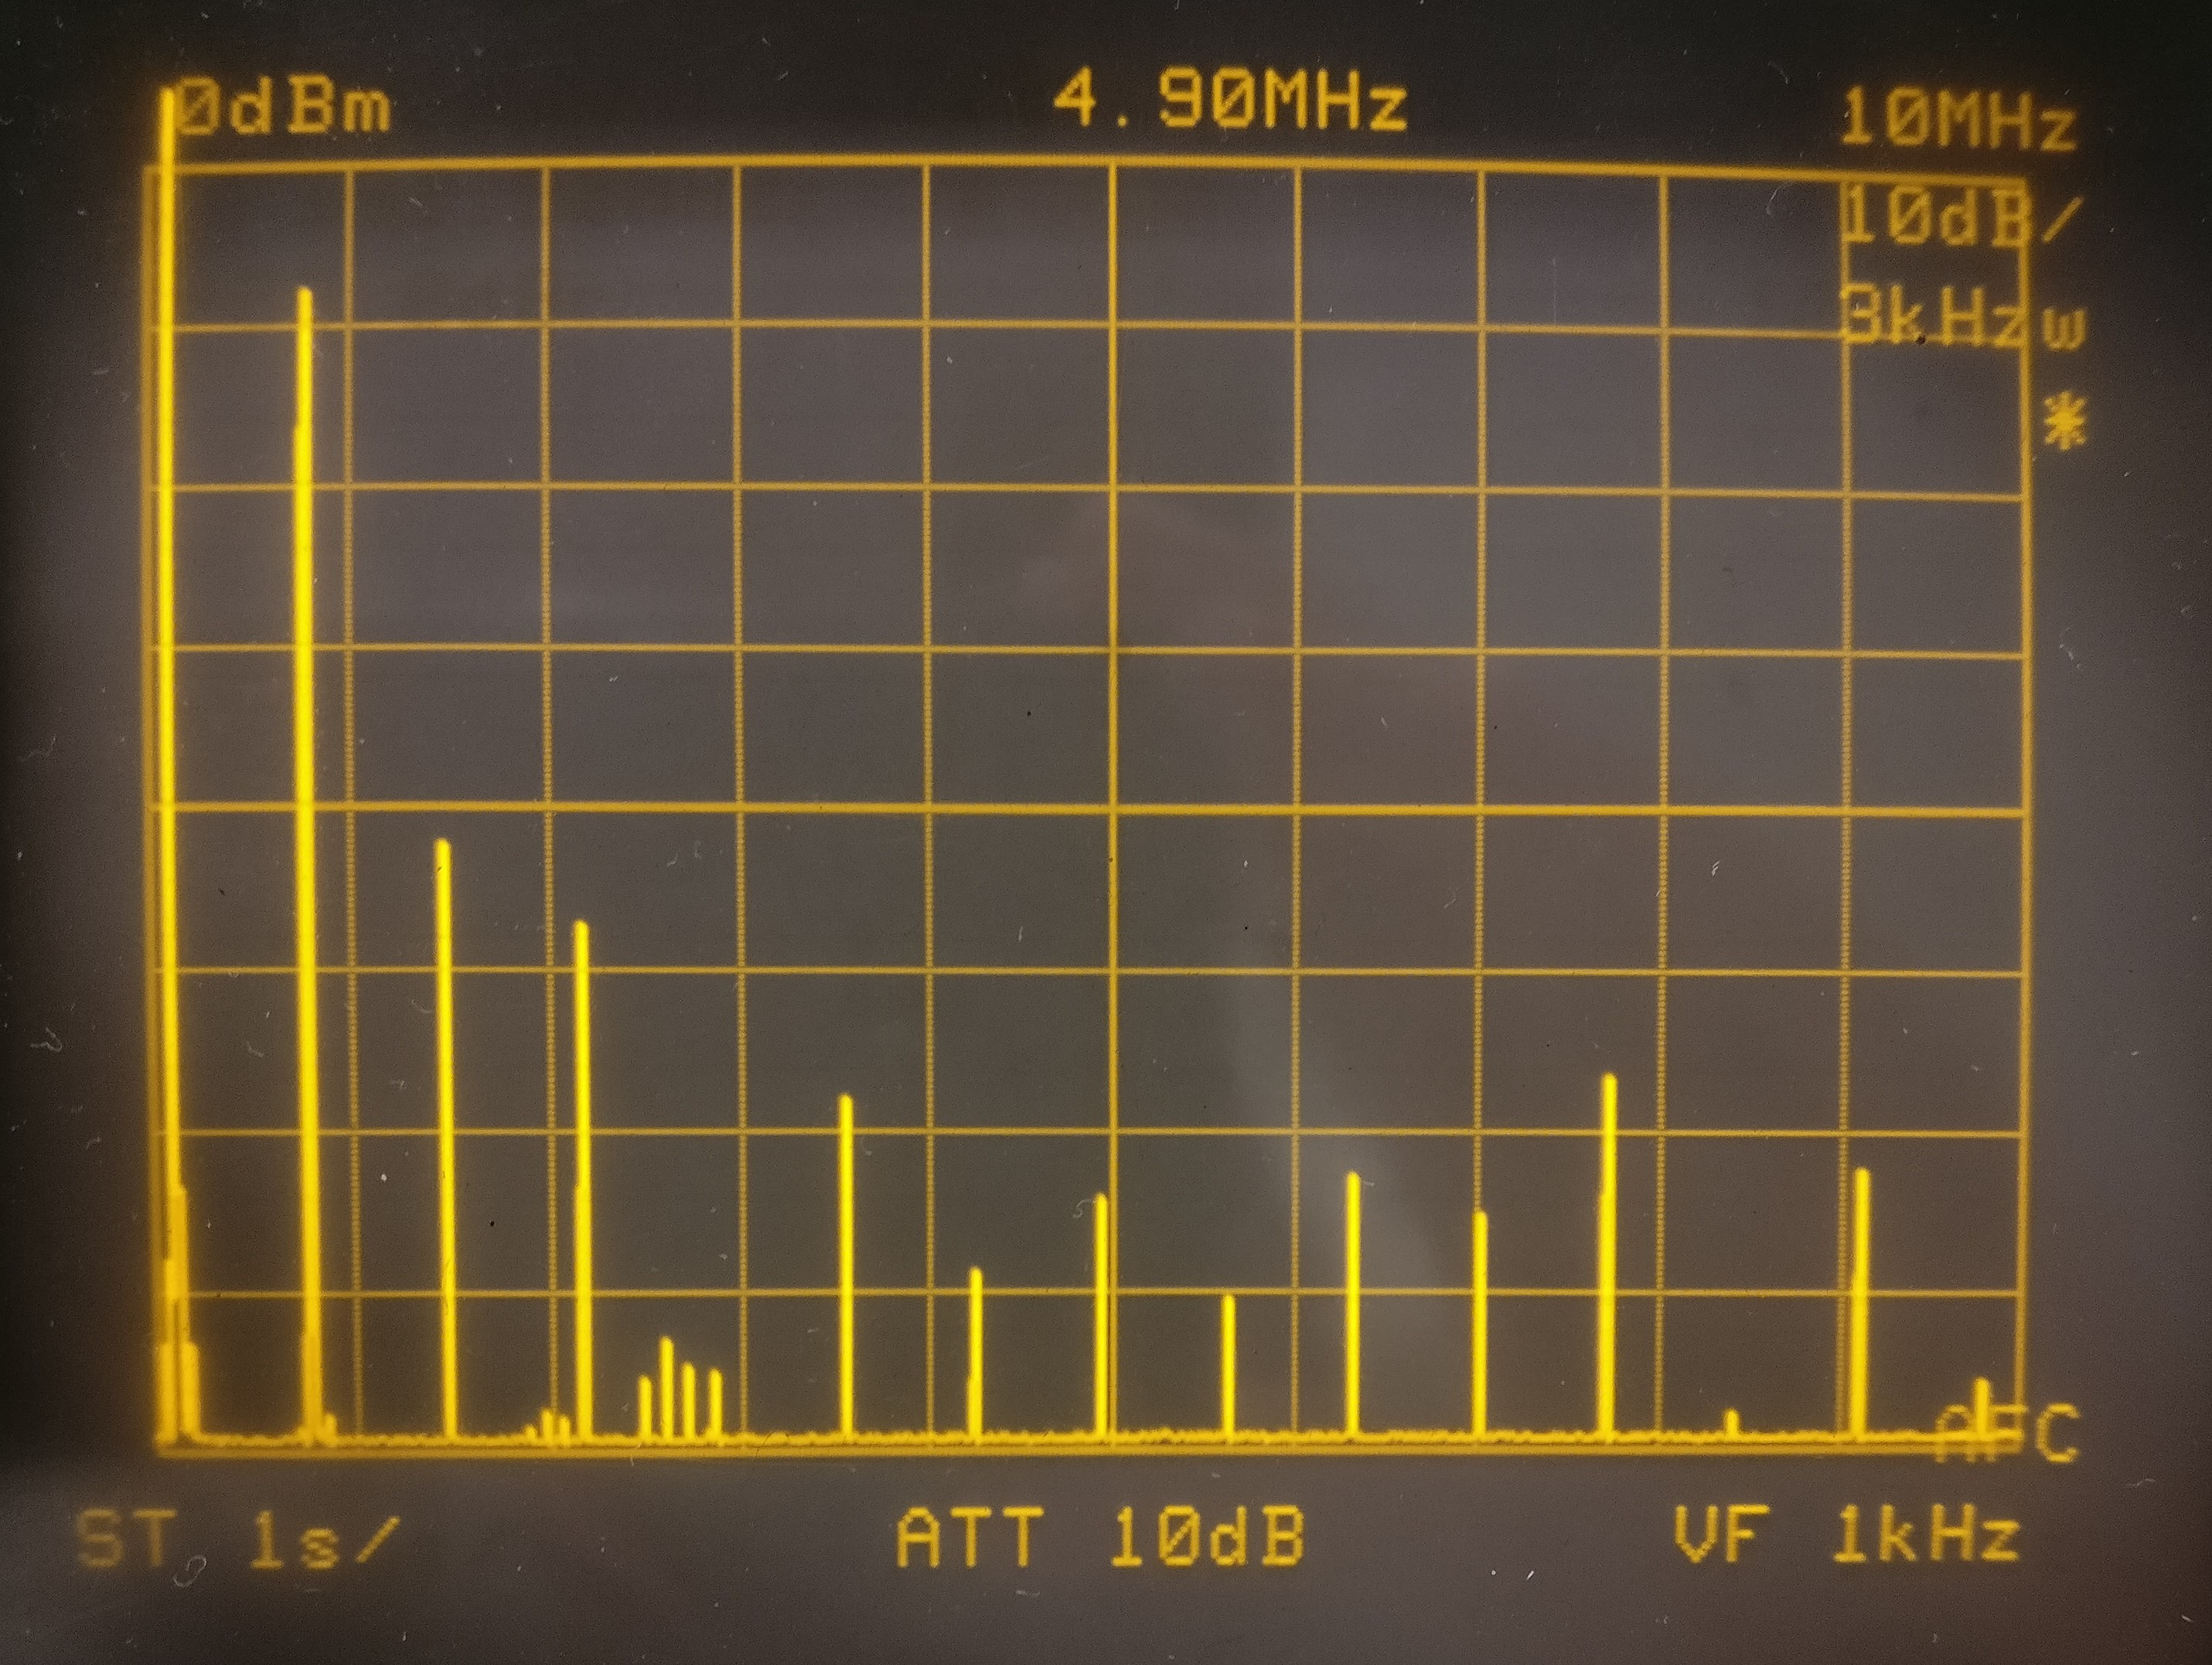
\includegraphics[width=0.5\linewidth]{contenido/img/espectro_instek}
        \caption{Espectro de la senoidal en el generador Instek}
        \label{fig:espectro_instek}
    \end{center}
\end{figure}

\section{Comparación con la hoja de datos y Conclusiones}
Observando los resultados de la tabla \ref{tab:ejmeas} se puede observar que, aunque en todos
los casos las distrociones armónicas son menores a las indicadas por las hojas de datos de los
fabricantes, el de Instek tiene un valor más cercano a este, además de ser de un orden de magnitud
mayor.

Dado esto, se puede verificas que la señal entregada por el generador Instek es de menor calidad,
ya que sufre mayor distorción, mientras que las señales entregadas por los generadores Picotest y Agilent
son de mejor calidad.